\documentclass[]{article}
\usepackage{lmodern}
\usepackage{amssymb,amsmath}
\usepackage{ifxetex,ifluatex}
\usepackage{fixltx2e} % provides \textsubscript
\ifnum 0\ifxetex 1\fi\ifluatex 1\fi=0 % if pdftex
  \usepackage[T1]{fontenc}
  \usepackage[utf8]{inputenc}
\else % if luatex or xelatex
  \ifxetex
    \usepackage{mathspec}
  \else
    \usepackage{fontspec}
  \fi
  \defaultfontfeatures{Ligatures=TeX,Scale=MatchLowercase}
\fi
% use upquote if available, for straight quotes in verbatim environments
\IfFileExists{upquote.sty}{\usepackage{upquote}}{}
% use microtype if available
\IfFileExists{microtype.sty}{%
\usepackage{microtype}
\UseMicrotypeSet[protrusion]{basicmath} % disable protrusion for tt fonts
}{}
\usepackage[margin=1in]{geometry}
\usepackage{hyperref}
\hypersetup{unicode=true,
            pdftitle={Trabalho de Econometria Espacial},
            pdfauthor={Bruno Tebaldi},
            pdfborder={0 0 0},
            breaklinks=true}
\urlstyle{same}  % don't use monospace font for urls
\usepackage{color}
\usepackage{fancyvrb}
\newcommand{\VerbBar}{|}
\newcommand{\VERB}{\Verb[commandchars=\\\{\}]}
\DefineVerbatimEnvironment{Highlighting}{Verbatim}{commandchars=\\\{\}}
% Add ',fontsize=\small' for more characters per line
\usepackage{framed}
\definecolor{shadecolor}{RGB}{248,248,248}
\newenvironment{Shaded}{\begin{snugshade}}{\end{snugshade}}
\newcommand{\KeywordTok}[1]{\textcolor[rgb]{0.13,0.29,0.53}{\textbf{#1}}}
\newcommand{\DataTypeTok}[1]{\textcolor[rgb]{0.13,0.29,0.53}{#1}}
\newcommand{\DecValTok}[1]{\textcolor[rgb]{0.00,0.00,0.81}{#1}}
\newcommand{\BaseNTok}[1]{\textcolor[rgb]{0.00,0.00,0.81}{#1}}
\newcommand{\FloatTok}[1]{\textcolor[rgb]{0.00,0.00,0.81}{#1}}
\newcommand{\ConstantTok}[1]{\textcolor[rgb]{0.00,0.00,0.00}{#1}}
\newcommand{\CharTok}[1]{\textcolor[rgb]{0.31,0.60,0.02}{#1}}
\newcommand{\SpecialCharTok}[1]{\textcolor[rgb]{0.00,0.00,0.00}{#1}}
\newcommand{\StringTok}[1]{\textcolor[rgb]{0.31,0.60,0.02}{#1}}
\newcommand{\VerbatimStringTok}[1]{\textcolor[rgb]{0.31,0.60,0.02}{#1}}
\newcommand{\SpecialStringTok}[1]{\textcolor[rgb]{0.31,0.60,0.02}{#1}}
\newcommand{\ImportTok}[1]{#1}
\newcommand{\CommentTok}[1]{\textcolor[rgb]{0.56,0.35,0.01}{\textit{#1}}}
\newcommand{\DocumentationTok}[1]{\textcolor[rgb]{0.56,0.35,0.01}{\textbf{\textit{#1}}}}
\newcommand{\AnnotationTok}[1]{\textcolor[rgb]{0.56,0.35,0.01}{\textbf{\textit{#1}}}}
\newcommand{\CommentVarTok}[1]{\textcolor[rgb]{0.56,0.35,0.01}{\textbf{\textit{#1}}}}
\newcommand{\OtherTok}[1]{\textcolor[rgb]{0.56,0.35,0.01}{#1}}
\newcommand{\FunctionTok}[1]{\textcolor[rgb]{0.00,0.00,0.00}{#1}}
\newcommand{\VariableTok}[1]{\textcolor[rgb]{0.00,0.00,0.00}{#1}}
\newcommand{\ControlFlowTok}[1]{\textcolor[rgb]{0.13,0.29,0.53}{\textbf{#1}}}
\newcommand{\OperatorTok}[1]{\textcolor[rgb]{0.81,0.36,0.00}{\textbf{#1}}}
\newcommand{\BuiltInTok}[1]{#1}
\newcommand{\ExtensionTok}[1]{#1}
\newcommand{\PreprocessorTok}[1]{\textcolor[rgb]{0.56,0.35,0.01}{\textit{#1}}}
\newcommand{\AttributeTok}[1]{\textcolor[rgb]{0.77,0.63,0.00}{#1}}
\newcommand{\RegionMarkerTok}[1]{#1}
\newcommand{\InformationTok}[1]{\textcolor[rgb]{0.56,0.35,0.01}{\textbf{\textit{#1}}}}
\newcommand{\WarningTok}[1]{\textcolor[rgb]{0.56,0.35,0.01}{\textbf{\textit{#1}}}}
\newcommand{\AlertTok}[1]{\textcolor[rgb]{0.94,0.16,0.16}{#1}}
\newcommand{\ErrorTok}[1]{\textcolor[rgb]{0.64,0.00,0.00}{\textbf{#1}}}
\newcommand{\NormalTok}[1]{#1}
\usepackage{longtable,booktabs}
\usepackage{graphicx,grffile}
\makeatletter
\def\maxwidth{\ifdim\Gin@nat@width>\linewidth\linewidth\else\Gin@nat@width\fi}
\def\maxheight{\ifdim\Gin@nat@height>\textheight\textheight\else\Gin@nat@height\fi}
\makeatother
% Scale images if necessary, so that they will not overflow the page
% margins by default, and it is still possible to overwrite the defaults
% using explicit options in \includegraphics[width, height, ...]{}
\setkeys{Gin}{width=\maxwidth,height=\maxheight,keepaspectratio}
\IfFileExists{parskip.sty}{%
\usepackage{parskip}
}{% else
\setlength{\parindent}{0pt}
\setlength{\parskip}{6pt plus 2pt minus 1pt}
}
\setlength{\emergencystretch}{3em}  % prevent overfull lines
\providecommand{\tightlist}{%
  \setlength{\itemsep}{0pt}\setlength{\parskip}{0pt}}
\setcounter{secnumdepth}{0}
% Redefines (sub)paragraphs to behave more like sections
\ifx\paragraph\undefined\else
\let\oldparagraph\paragraph
\renewcommand{\paragraph}[1]{\oldparagraph{#1}\mbox{}}
\fi
\ifx\subparagraph\undefined\else
\let\oldsubparagraph\subparagraph
\renewcommand{\subparagraph}[1]{\oldsubparagraph{#1}\mbox{}}
\fi

%%% Use protect on footnotes to avoid problems with footnotes in titles
\let\rmarkdownfootnote\footnote%
\def\footnote{\protect\rmarkdownfootnote}

%%% Change title format to be more compact
\usepackage{titling}

% Create subtitle command for use in maketitle
\providecommand{\subtitle}[1]{
  \posttitle{
    \begin{center}\large#1\end{center}
    }
}

\setlength{\droptitle}{-2em}

  \title{Trabalho de Econometria Espacial}
    \pretitle{\vspace{\droptitle}\centering\huge}
  \posttitle{\par}
    \author{Bruno Tebaldi}
    \preauthor{\centering\large\emph}
  \postauthor{\par}
      \predate{\centering\large\emph}
  \postdate{\par}
    \date{April 11, 2019}


\begin{document}
\maketitle

\url{https://rmarkdown.rstudio.com/authoring_bibliographies_and_citations.html}

\subsection{R Markdown}\label{r-markdown}

Resumo \#\# Introducao e revisao bibliografica

Econometric studies of unemployment with a regional dimension often
consist of papers using individual level data to explain how regional
factors affect employment outcomes alongside individual characteristics.

Firstly, focusing on the Brazilian labor market, Oliveira and Carneiro
{[}2001{]} analyzed the fluctuations in the employment level of several
Brazilian states compared to national employment. The purpose of their
study was to verify whether it is possible to establish a long-term
relationship between state employment and nationwide employment. To
achieve this the authors applied a cointegration analysis, a methodology
proposed by Engle and Granger {[}1987{]}, as well as the model of
unrestricted error correction as proposed by Pesaran et al. {[}1996{]}.
The results obtained from an Vector Error Correction model were
consistent with those obtained with Engle and Granger method (Engle and
Granger {[}1987{]}). The results lead to the conclusion that employment
fluctuations in most states shares a common trend with national
employment level.

The hypothesis that the formal labor market presents a different
dynamics in Brazilian metropolitan and nonmetropolitan areas was tested
by Kretzmann and da Cunha {[}2009{]}. The goal of their study was to
analyze the fluctuations in the labor market of metropolitan and
non-metropolitan Brazilian areas. They used employment and unemployment
data from the Ministry of Labor and Employment through the General
Records of Employed and Unemployed Persons - CAGED - using monthly data
from 1996 through 2007. Kretzmann and da Cunha {[}2009{]} used
cointegration analysis through the traditional method proposed by
Engle-Granger, as well as the method proposed by Pesaran et al.
{[}1996{]}. The two methods produced the similar results, suggesting
that the metropolitan and non-metropolitan areas are not co-integrated.

None of these paper deals with the curse of dimensionality. The authors
opt to with pairs of series. The evidence that states and national share
a common trend highlight a possible channel linking macro and regional
dynamics.

Althought this body of past research can offer a number of useful
insights, however, none of these papers establishes the presence of
spatial dependence nor it aims to identify the spatial interdependence
between the regions.

Addressing these gaps is important as unemployment has significant
consequences at both the micro and macro levels. For individuals, being
unemployed can result in lowered income and possibly self-esteem, while
at the macro level, elevated unemployment levels entail a loss of
economic output and raised welfare spending (Brown and Sessions, 1997).
This problem of a lack of understanding eventual spatial dependencies
affecting unemployment in Brazil presents a clear motivation for
carrying out this study.

\subsection{Research Questions}\label{research-questions}

Como mencionado anteriormente, pretendemos modelar o fluxo de emprego
liquido levando em conta as dependências espaciais. Além disso, como
objetivo secundário, pretendemos comparar dois duas métricas utilizadas
para a construção da matrix de pessos utilizados na modelagem espacial.

\subsection{Model ???}\label{model}

A utilização dos modelos espaciais é indicada quando existe a interação
entre regiões com uma uma persistência no espaço das caracteristicas
observadas. Neste cenário, a utilização de econometria espcacial leva em
conta não somente a influencia das variaveis independentes, mas também
os efeitos das vizinhanças. Esse efeito de regional das vizinhancas é
capturado por meio de uma matriz de pesos o qual é responsavel por
capturar o efeito de defazagem espacial. Primeiramente vamos analisar o
fluxo de emprego liquido, logo teremos que para cada região \(s\), a
variável \(y(s)\) será definida pelo fluxo de emprego líquido, sendo
assim \(y(s)\) será aquantidade de pessoas admitidas no mercado de
trabalho menos a quantidade de pessoas desligadas do mercado de
trabalho.

Referente a matriz de pessos é na realidade uma métrica da distancia
entre as regiões, aonde vale resaltar que essa métrica não precisa estar
associada a espaço físico, podendo ser uma métrica econômica, política
ou social, etc.

Sendo assim vamos utilizar dois modelos esaciais, o modelo
autoregressivo espacial (SAR) e o modelo autoregressivos espaciais
Condicional (CAR)

\paragraph{Modelo SAR}\label{modelo-sar}

Designaremos cada localidade por \(S_i\), e um conjunto de vizinhos
\(N(S_i)\). Sendo assim, definimos o modelo Autoregressivo espacial
(SAR) como

\begin{equation}
  y(s) = \delta + X(s)\beta + \phi \frac{1}{\left| N(s) \right|} \sum_{s' \in N(s)} y(s') + \mathcal{N}(0,\sigma^2)
\end{equation}

Aonde \(X(s)\) é um vetor de covariadas, o parâmetro autoregressivo
espacial é ponderado por uma média dos valores dos vizinhos (tal como
especificada pela matriz de vizinhança). O modelo pode ser reescrito
como:

\begin{equation}
  y(s) = \delta + X(s)\beta + \phi \sum_{s' \in N(s)} \frac{W_{s, s'}}{W_s}  y(s') + \epsilon
\end{equation}

aonde \(\epsilon \sim \mathcal{N}(0,\sigma^2 I)\)

\paragraph{Modelo CAR}\label{modelo-car}

Seguindo a mesma terminologia, o modelo autoregressivo espacial da forma
condicional pode ser escrito como:
\[y(s)|y_{-s} \sim \mathcal{N}\left(\sum_{s'} \frac{W_{s, s'}}{W_s} y(s'), \sigma^2 \right)\]

Portanto, a distribuição dos atributos em um modelo CAR é \$ y
\sim \mathcal{N}\left(0, \sigma\^{}2\left( I - \phi W
\right)\^{}\{-1\}\right)\$

\subsection{Matrix de peso Modelo}\label{matrix-de-peso-modelo}

o critério de escolha de vizinhanças possui um impacto fundamental nos
resultados das estatísticas descritivas.

A especificação da matrix de pessos, \(W\), é tipicamente baseada em
alguma medida de distância entre regiões. No nosso estudo vamos utilizar
dois tipos de métricas. A primeira métrica é a usualmente usada na
literatura, tambem conhecido como queen. A segunda metrica é baseado no
número de conexoes fisicas (ruas, estradas, vias aéreas, vias fluviais,
etc) entre regioes.

\subsubsection{Matrix Queen}\label{matrix-queen}

As linhas e colunas dessa matriz, frequentemente denotadas por
\(W = (w_{ij})\), correspondem às observações de corte transversal (por
exemplo, indivíduos, regiões ou países), e o elemento genérico,
\(w_{ij}\), pode ser interpretado como a força da potencial interação
entre as unidades \(i\) e \(j\).

Essa matriz de pesso e baseada na posição geograffica entre as regioes.
Ela é uma matriz de contiguidade binária, tendo seu elementos \((i, j)\)
igual a ``um'' ou ``zero''. Se duas regiões são vizinhas, o valor será
igual a ``um'' caso contrário será atribuído o valor igual ``zero''.

Desta forma teremos que a matriz de pesos espaciais pode ser definida
como :

\[w_{ij} = \begin{cases} 1 & \text{se } i \text{ e } j \text{ são conectadas} \\ 0 & \text{caso contrário} \end{cases}\]

\subsubsection{Matrix de Conexoes}\label{matrix-de-conexoes}

A matriz de pesos deve ser definida de modo que \(W\) capture a
persistência das variáveis em outras regiões. Assim, para determinar a
matriz de peso, é necessário determinar a importância de cada região em
relação a todas as outras regiões.

Focando no mercado de trabalho, determinar a importância de uma região
em relacao a outra, é determinar a importância de um mercado de trabalho
em relação a outro mercado de trabalho. Cada região tem seu próprio
mercado de trabalho com empresas e trabalhadores, e como as empresas não
podem mudar de mercado, são os trabalhadores que mudam livremente de
mercado. Em outras palavras, um trabalhador pode procurar emprego em
outras regiões, mas uma empresa deve atrair trabalhadores de outras
regiões para seu próprio mercado. Conseqüentemente, para um trabalhador
viajar para outra região, deve haver uma conexão entre essas regiões.

A matriz de peso, pode então, ser determinada pelo número de conexões
entre as regiões dividido pelo seu número total de conexões. Portanto,
para cada regiao \(s\) o vetor de peso \(W_s\) associado a essa regiao é
determinado como:

\[W_i = \frac{\left[C_{s, 1}, \dots C_{s, n}\right]}{\sum_{s'} C_{s, s'}}a \]

aonde \(C_{i, j}\) é o número de conexoes entre a regiao \(i\) e regiao
\(j\), e \(n\) é quantidade total de regiões.

\subsection{Variaveis de controle}\label{variaveis-de-controle}

Diversos fatores podem influenciar o fluxo de empregos de uma região.
Por exemplo, é esperado que uma região com uma maior concentração de
industrias tenha um maior nivel de emprego e consequentemente um maior
fluxo no emprego. Apresentamos aqui alguns dos fatores que consideramos
importantes.

\subsubsection{Demografia}\label{demografia}

A estrutura etária pode influenciar a taxa de desemprego de uma área
através de seu impacto no comportamento de busca, já que os jovens
trabalhadores têm maior probabilidade de mudar de emprego em busca de um
emprego melhor, enquanto trabalhadores mais velhos já tiveram a chance
de passar por esse processo e favorecem empregos mais estaveis (Brown \&
Sessions, 1997). Isto sugere que áreas com muitos trabalhadores jovens
deverão ter um fluxo de emprego mais elevado.

\subsubsection{2.6.5. Mix de firmas}\label{mix-de-firmas}

O mix de indústria de uma região pode influenciar o comportamento de
busca e, portanto, o desemprego. Além do canal de de oferta de vagas, o
qual influencia diretamente a taxa de emprego, existe outro canal de
impacto relacionado as firmas, este canal vem de mudanças no mix das
firmas que podem aumentar o desemprego. Isso pode ocorrer devido à
mudanças na estrutura industrial o qual podem significar que as
habilidades dos candidatos ao emprego não são adequadas às vagas
oferecidas, de modo que ocorre um aumento na taxa de desemprego.

\subsubsection{Criminalidade}\label{criminalidade}

A literatura econômica sugere que a atividade criminosa é motivada
principalmente pelos benefícios relativos a atividades ilegais. Primeiro
apontado por Becker (1968), criminosos em potencial pesam os custos e os
benefícios de cometer crimes. Indivíduos podem gerar renda através de
atividades criminosas e mercados de trabalho. Consequentemente, a renda
obtida em uma dessas alternativas é incluída no custo de participação na
outra (Block e Heineke, 1975, Ehrlich, 1973, Machin e Meghir, 2004,
Mocan et al., 2005). Indivíduos com oportunidades atuais e futuras
potencialmente melhores no mercado de trabalho legal são menos propensos
a cometer crimes.

Um fator determinante dessas oportunidades no mercado de trabalho é a
taxa de desemprego, que flutua ao longo do ciclo econômico. Durante uma
recessão, quando a taxa de desemprego aumenta, as chances de emprego no
mercado de trabalho legal diminuem, neste cenário, enquanto as
perspectivas de emprego dos indivíduos forem influenciadas pelas
condições legais do mercado de trabalho, as mudanças na taxa de
desemprego terão impacto na taxa de criminalidade, que é uma agregação
das atividades criminosas dos indivíduos. Em tempos de desemprego
elevado, o benefício relativo de trabalhar no mercado de trabalho legal
para um indivíduo diminui na margem, aumentando a taxa de criminalidade
no país.

\subsubsection{Capital humano}\label{capital-humano}

Espera-se que os indivíduos com níveis mais altos de capital humano
sejam mais consistentemente demandados pelos empregadores bem como é
esperado que indivíduos com níveis mais altos de capital humano realizem
pesquisas de emprego mais eficientes (Elhorst, 2003). Isso significa que
áreas com uma alta proporção de indivíduos com níveis mais altos de
capital humano devem ter taxas de desemprego mais baixas.

\subsubsection{Moradia}\label{moradia}

O status de moradia pode afetar o comportamento de busca e, portanto, o
desemprego de várias maneiras, por exemplo, os residentes em moradias
públicas podem relutar em mudar de região em busca de emprego. Isso pode
ser porque receber um lugar em moradias públicas é efetivamente um
subsídio (Brown and Sessions, 1997) e a perspectiva de perder este
subsídio, mudando para um novo emprego, pode tornar as buscas de
residentes de moradias de moradia mais restritas. O mesmo também pode
ser verdade para os ocupantes-proprietários, dados os custos de
transação associados à compra da casa.

\subsubsection{Beneficios sociais}\label{beneficios-sociais}

O valor real dos benefícios de desemprego pode afetar as taxas de
emprego e desemprego, aumentando o salário de reserva dos candidatos à
emprego, reduzindo a atratividade de conseguir um novo emprego (Elhorst,
2003). Mesmo que tais benefícios sejam estabelecidos nacionalmente, se
isso for feito em termos nominais, eles podem ter um impacto em nível
regional se os diferentes custos de vida significarem que seu valor real
varia. Little (2009)

\subsection{Descricao da base de
dados}\label{descricao-da-base-de-dados}

Este capítulo apresentará a base de dados utilizada.

O objetivo deste trabalho é analisar o fluxo de emprego líquido no
estado de São Paulo, levando em consideração os efeitos espaciais. Para
isso serão utilizado duas métricas de distancia, e será feito o controle
por diversas covariadas.

O estado de São Paulo é formado por 644 municípios (município de
Ilhabela foi desconsiderado da amostra devido ser uma região sem
vizinhos). A variável dependente é o fluxo de emprego líquido,
construído a partir do fluxo formal de admisão e desligamentos no
mercado de trabalho, com dados obtidos do Cadastro Geral de Empregados e
Desempregados (CAGED).

As demais variáveis explicativas utilizadas no modelo foram obtidos no
site da Fundação SEADE e estão descritas conforme a seguir:

\begin{longtable}[]{@{}ll@{}}
\caption{Tabela de descricao dos dados}\tabularnewline
\toprule
Cod. Variavel & Descricao\tabularnewline
\midrule
\endfirsthead
\toprule
Cod. Variavel & Descricao\tabularnewline
\midrule
\endhead
CodIbge & Código do IBGE para o municipio\tabularnewline
Anaf & Taxa de Analfabetismo da População de 15 Anos e Mais - Censo
Demográfico (Em \%)\tabularnewline
Educ & População de 18 a 24 Anos com pelo Menos Ensino Fundamental
Completo - Censo Demográfico (Em \%)\tabularnewline
Power & Consumo de Energia Elétrica - Total (Em MWh)\tabularnewline
Idh & Índice de Desenvolvimento Humano Municipal - IDHM\tabularnewline
Furto & Total Ocorrências de Furtos\tabularnewline
PIB\_pc & PIB per Capita (Em reais correntes)\tabularnewline
Agric & Valor Adicionado da Agropecuária (Em mil reais
correntes)\tabularnewline
Saude & Total de Despesas Municipais - Saúde (Em reais de
2018)\tabularnewline
Longevidade & Índice de Desenvolvimento Humano Municipal - IDHM
Longevidade\tabularnewline
Gini & O índice de Gini\tabularnewline
Crime & Crime\tabularnewline
educ & educ\tabularnewline
PIB & Produto interno bruto da regiao\tabularnewline
Adm & Adm\tabularnewline
Desl & Desl\tabularnewline
\bottomrule
\end{longtable}

\subsection{Resultados}\label{resultados}

Esta seção apresentamos o procedimento para execução das regressoes bem
como os resultados obtidos.

Nosso primeiro passo é carregar todas as bibliotecas que iremos utilizar
no estudo

\begin{Shaded}
\begin{Highlighting}[]
\KeywordTok{source}\NormalTok{(}\StringTok{"./InstallPackages.R"}\NormalTok{)}
\end{Highlighting}
\end{Shaded}

\begin{verbatim}
## [1] "Loading the folowiong libraries: sp, ggmap, tidyverse, magrittr, gstat, latex2exp, spdep, sf, readxl, raster, GISTools, knitr"
\end{verbatim}

Temos a base de dados agrupado separadamente do nosso \emph{shapefile}
então carregamos separadamente cada um dos arquivos.

\begin{Shaded}
\begin{Highlighting}[]
\CommentTok{# carrega o shapefile }
\NormalTok{municipios <-}\StringTok{ }\NormalTok{sf}\OperatorTok{::}\KeywordTok{st_read}\NormalTok{(}\StringTok{"./ShapeFile/35MUE250GC_SIR.shp"}\NormalTok{)}
\end{Highlighting}
\end{Shaded}

\begin{verbatim}
## Reading layer `35MUE250GC_SIR' from data source `C:\Users\Tebaldi\Documents\GitHub\EconometriaEspacial\ShapeFile\35MUE250GC_SIR.shp' using driver `ESRI Shapefile'
## Simple feature collection with 645 features and 3 fields
## geometry type:  MULTIPOLYGON
## dimension:      XY
## bbox:           xmin: -53.11011 ymin: -25.31232 xmax: -44.16137 ymax: -19.77966
## epsg (SRID):    NA
## proj4string:    +proj=longlat +ellps=GRS80 +no_defs
\end{verbatim}

\begin{Shaded}
\begin{Highlighting}[]
\CommentTok{# carrega o a base de dados}
\NormalTok{dados <-}\StringTok{ }\KeywordTok{read_excel}\NormalTok{(}\StringTok{"./Dados.xlsx"}\NormalTok{)}
\end{Highlighting}
\end{Shaded}

\begin{verbatim}
## New names:
## * `` -> ...1
\end{verbatim}

\begin{Shaded}
\begin{Highlighting}[]
\CommentTok{# Impressao do mapa utilizando o ggplot2}
\KeywordTok{ggplot}\NormalTok{(municipios) }\OperatorTok{+}\StringTok{ }\KeywordTok{geom_sf}\NormalTok{()}
\end{Highlighting}
\end{Shaded}

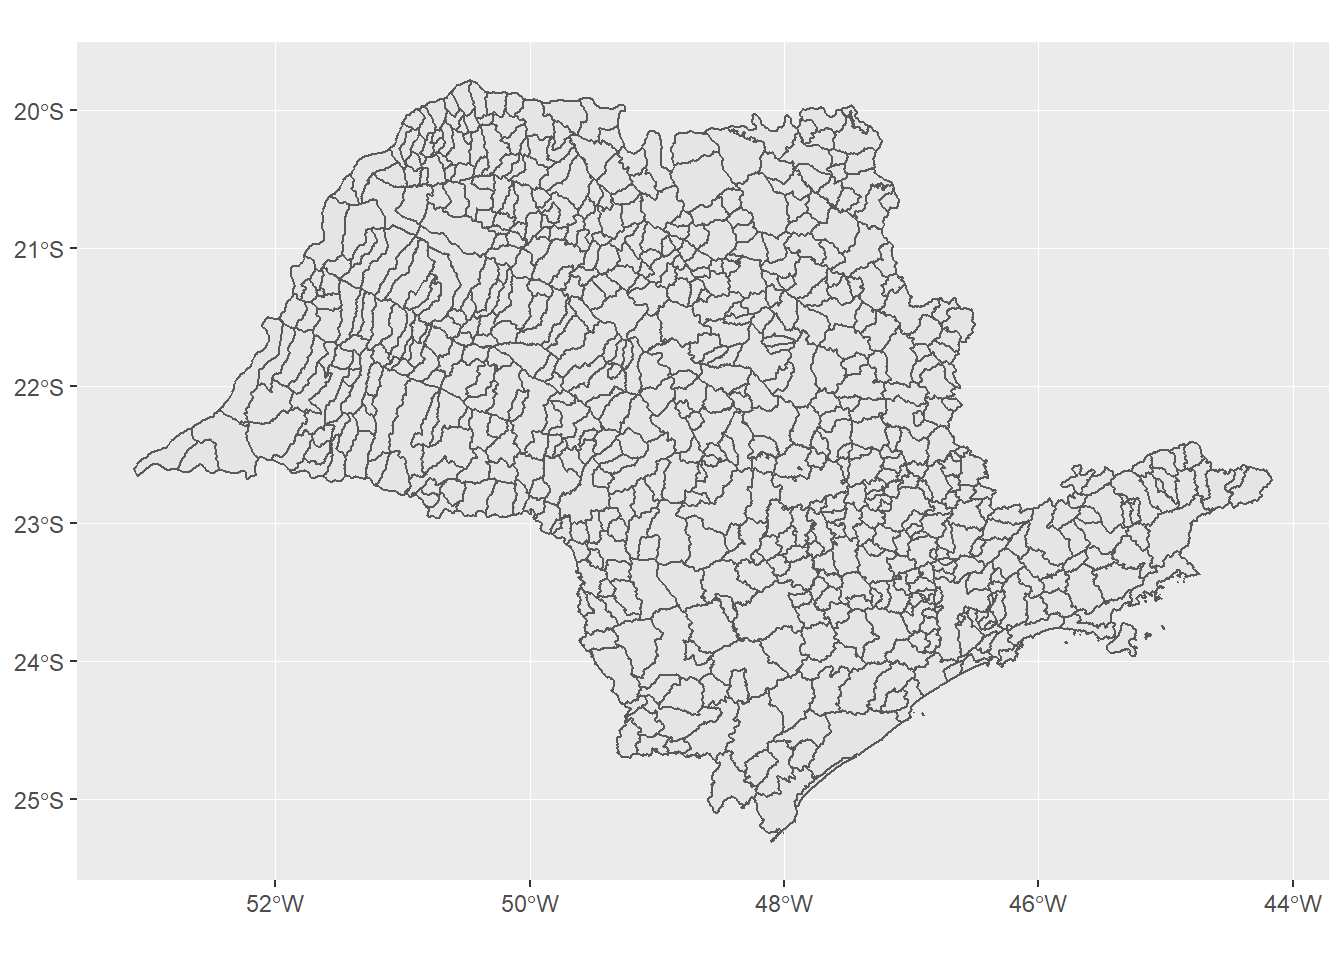
\includegraphics{trabalho_files/figure-latex/unnamed-chunk-3-1.pdf}

A base de dados é anexada ao shapefile por meio do pacote dplyr.

\begin{Shaded}
\begin{Highlighting}[]
\CommentTok{# Verifica as diferencas entre as base de dados}
\CommentTok{# Dados que estao na base de dados de criminalidade}
\CommentTok{# menos os municipios do shapefile}
\NormalTok{dplyr}\OperatorTok{::}\KeywordTok{setdiff}\NormalTok{(dados}\OperatorTok{$}\NormalTok{CodIbge, municipios}\OperatorTok{$}\NormalTok{CD_GEOCMU)}
\end{Highlighting}
\end{Shaded}

\begin{verbatim}
## numeric(0)
\end{verbatim}

\begin{Shaded}
\begin{Highlighting}[]
\CommentTok{# Dados que estao na base do shapelife}
\CommentTok{# menos os municipios na base de dados de criminalidade}
\NormalTok{dplyr}\OperatorTok{::}\KeywordTok{setdiff}\NormalTok{(municipios}\OperatorTok{$}\NormalTok{CD_GEOCMU, dados}\OperatorTok{$}\NormalTok{CodIbge)}
\end{Highlighting}
\end{Shaded}

\begin{verbatim}
## numeric(0)
\end{verbatim}

\begin{Shaded}
\begin{Highlighting}[]
\CommentTok{# Faz um merge dos dados em uma unica base de dados}
\NormalTok{Dados.sp <-}\StringTok{ }\NormalTok{dplyr}\OperatorTok{::}\KeywordTok{full_join}\NormalTok{(municipios, dados,  }\DataTypeTok{by =} \KeywordTok{c}\NormalTok{(}\StringTok{"CD_GEOCMU"}\NormalTok{ =}\StringTok{ "CodIbge"}\NormalTok{))}
\end{Highlighting}
\end{Shaded}

This is an R Markdown document. Markdown is a simple formatting syntax
for authoring HTML, PDF, and MS Word documents. For more details on
using R Markdown see \url{http://rmarkdown.rstudio.com}.

When you click the \textbf{Knit} button a document will be generated
that includes both content as well as the output of any embedded R code
chunks within the document. You can embed an R code chunk like this:

In many cases, it is common to assume that observations are independent
and identically distributed, but this may not be the case when working
with spatial data.

Observations are not independent because there may exist some
correlation between neighbouring areas. It may also be difficult to pick
apart the impact of spatial autocorrelation and spatial differences in
the distribution of the observation.

Cressie (1993, pp.~402--448, 458--477, 548-- 568) provides a very wide
discussion of these approaches, including reviews of the background for
their development and comprehensive worked examples. Schabenberger and
Gotway (2005, pp.~335--348) and Waller and Gotway (2004, pp.~362--380)
concentrate on the spatial autoregressive models to be used in this
section.

From a statistical point of view, it is possible to account for
correlated observations by considering a structure of the following kind
in the model. If the vector of response variables is multivariate
normal, we can express the model as follows:

\begin{equation}
Y = \mu +e
\end{equation}

where \(\mu\) is the vector of area means, which can be modelled in
different ways and \(e\) is the vector of random errors, which we assume
is normally distributed with zero mean and generic variance \(V\).

The mean is often supposed to depend on a linear term on some covariates
X, so that we will substitute the mean by \(X^T\beta\) in the model. On
the other hand, correlation between areas is taken into account by
considering a specific form of the variance matrix V .

\begin{Shaded}
\begin{Highlighting}[]
\KeywordTok{source}\NormalTok{(}\StringTok{"./InstallPackages.R"}\NormalTok{)}
\end{Highlighting}
\end{Shaded}

\begin{verbatim}
## [1] "Loading the folowiong libraries: sp, ggmap, tidyverse, magrittr, gstat, latex2exp, spdep, sf, readxl, raster, GISTools, knitr"
\end{verbatim}

\begin{Shaded}
\begin{Highlighting}[]
\CommentTok{# carrega shapefile}
\NormalTok{municipios <-}\StringTok{ }\NormalTok{sf}\OperatorTok{::}\KeywordTok{st_read}\NormalTok{(}\StringTok{"./ShapeFile/35MUE250GC_SIR.shp"}\NormalTok{)}
\end{Highlighting}
\end{Shaded}

\begin{verbatim}
## Reading layer `35MUE250GC_SIR' from data source `C:\Users\Tebaldi\Documents\GitHub\EconometriaEspacial\ShapeFile\35MUE250GC_SIR.shp' using driver `ESRI Shapefile'
## Simple feature collection with 645 features and 3 fields
## geometry type:  MULTIPOLYGON
## dimension:      XY
## bbox:           xmin: -53.11011 ymin: -25.31232 xmax: -44.16137 ymax: -19.77966
## epsg (SRID):    NA
## proj4string:    +proj=longlat +ellps=GRS80 +no_defs
\end{verbatim}

\begin{Shaded}
\begin{Highlighting}[]
\CommentTok{# Carrega dados de criminalidade}
\NormalTok{dados.crim.}\DecValTok{2010}\NormalTok{ <-}\StringTok{ }\KeywordTok{read_excel}\NormalTok{(}\StringTok{"./dados_crim_sp_2010.xlsx"}\NormalTok{)}
\end{Highlighting}
\end{Shaded}

\begin{Shaded}
\begin{Highlighting}[]
\KeywordTok{ggplot}\NormalTok{(municipios) }\OperatorTok{+}\StringTok{ }\KeywordTok{geom_sf}\NormalTok{()}
\end{Highlighting}
\end{Shaded}

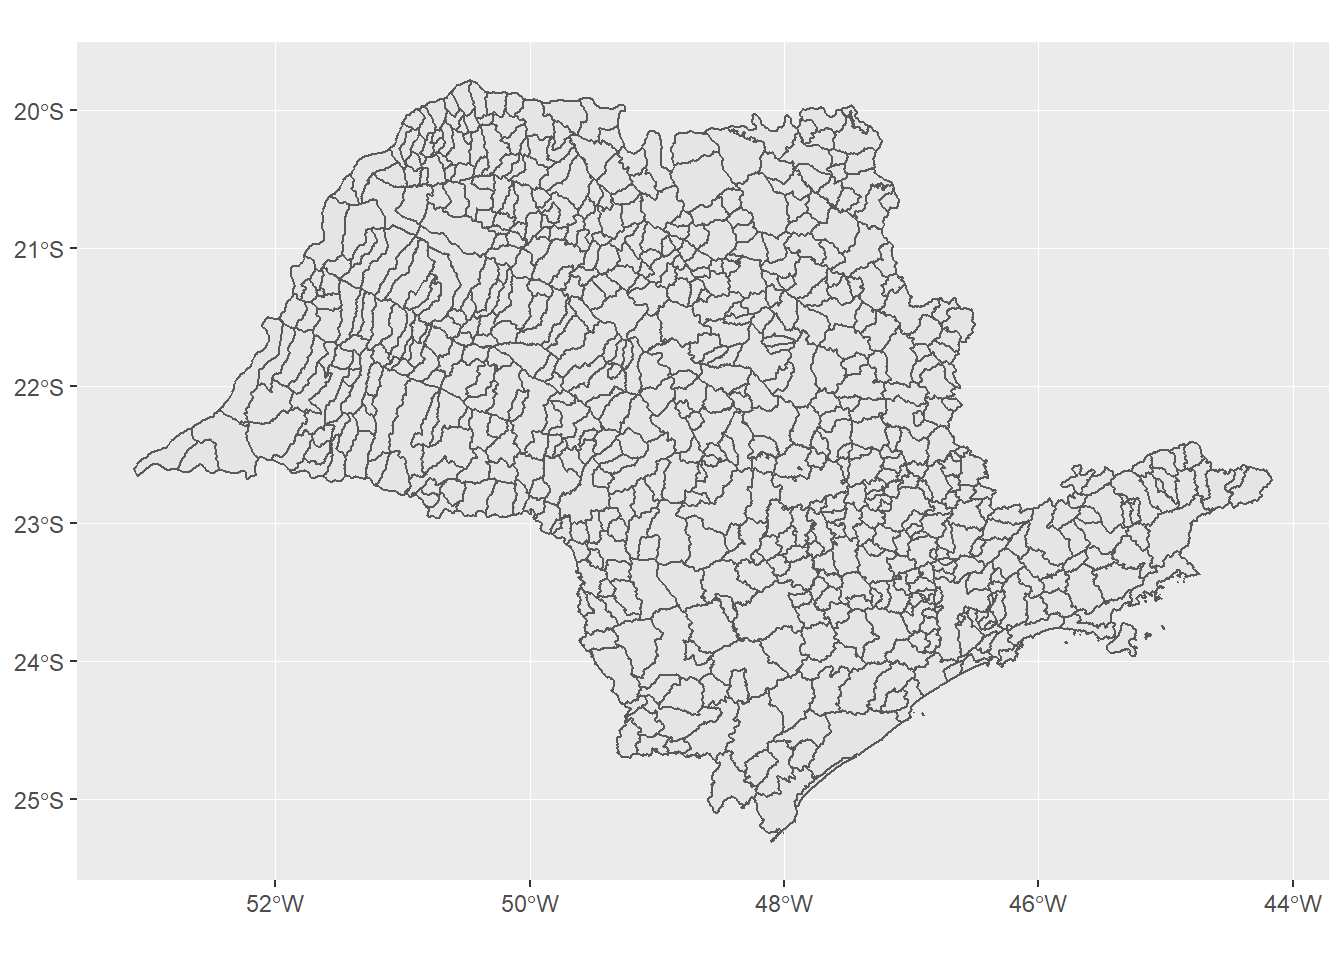
\includegraphics{trabalho_files/figure-latex/unnamed-chunk-5-1.pdf}

\begin{Shaded}
\begin{Highlighting}[]
\NormalTok{dplyr}\OperatorTok{::}\KeywordTok{setdiff}\NormalTok{(dados.crim.}\DecValTok{2010}\OperatorTok{$}\NormalTok{CodIBGE, municipios}\OperatorTok{$}\NormalTok{CD_GEOCMU)}
\end{Highlighting}
\end{Shaded}

\begin{verbatim}
## numeric(0)
\end{verbatim}

\begin{Shaded}
\begin{Highlighting}[]
\CommentTok{# Dados que estao na base do shapelife}
\CommentTok{# menos os municipios na base de dados de criminalidade}
\NormalTok{dplyr}\OperatorTok{::}\KeywordTok{setdiff}\NormalTok{(municipios}\OperatorTok{$}\NormalTok{CD_GEOCMU, dados.crim.}\DecValTok{2010}\OperatorTok{$}\NormalTok{CodIBGE)}
\end{Highlighting}
\end{Shaded}

\begin{verbatim}
## [1] 3505351 3507209 3509957 3531001
\end{verbatim}

\begin{Shaded}
\begin{Highlighting}[]
\CommentTok{# Faz um merge dos dados em uma unica base de dados}
\NormalTok{crim.sp <-}\StringTok{ }\NormalTok{dplyr}\OperatorTok{::}\KeywordTok{full_join}\NormalTok{(municipios, dados.crim.}\DecValTok{2010}\NormalTok{,  }\DataTypeTok{by =} \KeywordTok{c}\NormalTok{(}\StringTok{"CD_GEOCMU"}\NormalTok{ =}\StringTok{ "CodIBGE"}\NormalTok{))}
\end{Highlighting}
\end{Shaded}

\subsection{Including Plots}\label{including-plots}

You can also embed plots, for example:

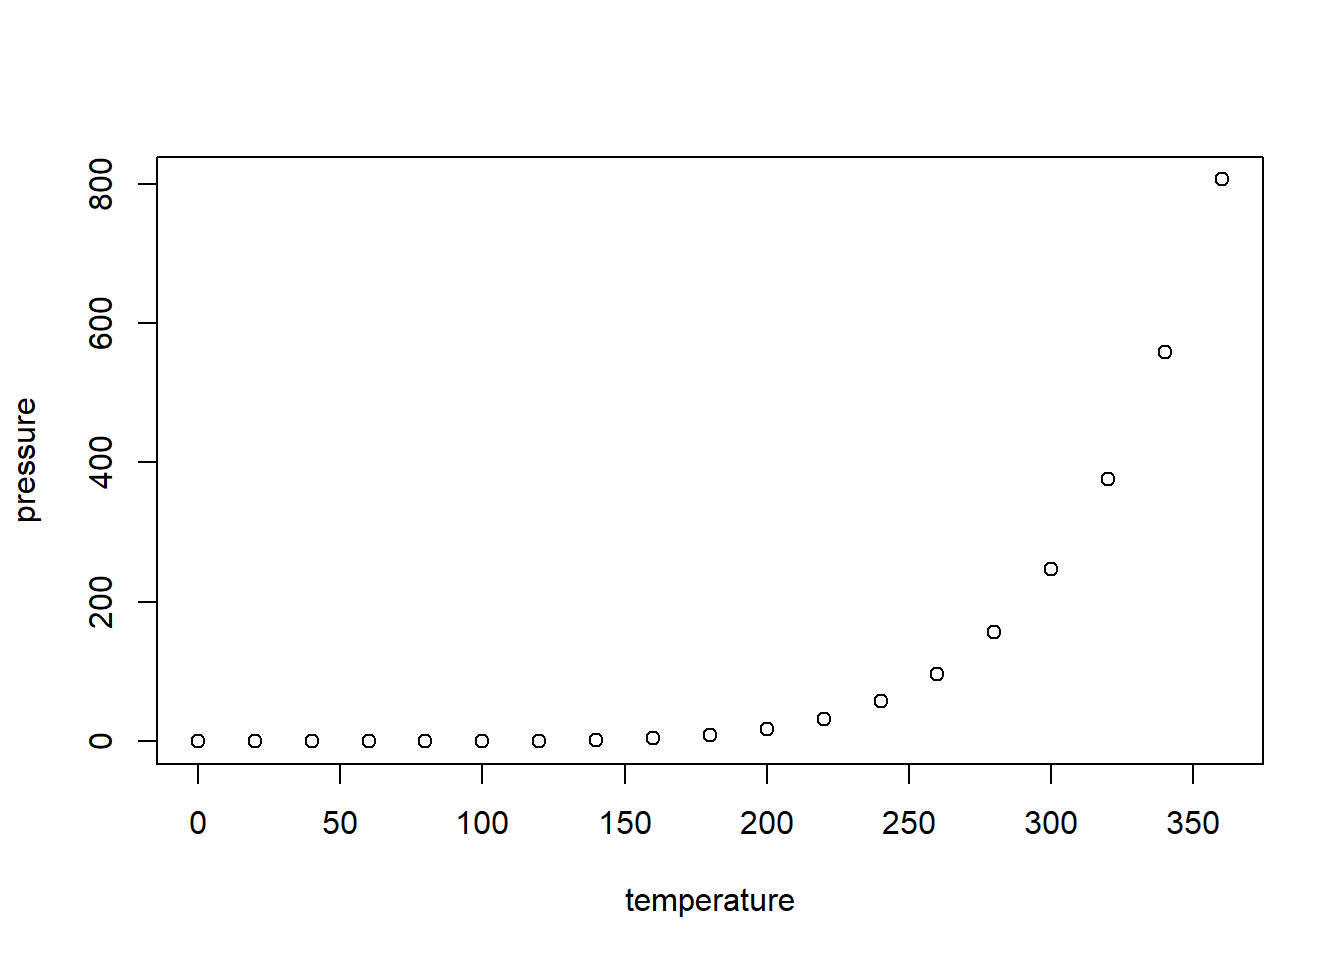
\includegraphics{trabalho_files/figure-latex/pressure-1.pdf}

Note that the \texttt{echo\ =\ FALSE} parameter was added to the code
chunk to prevent printing of the R code that generated the plot.

International Review of Law and Economics Volume 32, Issue 1, March
2012, Pages 145-157


\end{document}
